\documentclass[pdf, handout]{beamer}
\usepackage{tikz} 
\usepackage{amsmath}
\usepackage{amsthm}
\usepackage{amssymb}              % used for \eqref{} in this document
\usepackage{dsfont}
\usepackage{hyperref}
\DeclareMathOperator*{\argmin}{arg\,min}
\mode<presentation>{\usetheme{Malmoe}}
\usecolortheme{beaver}
\usepackage{graphicx}
\graphicspath{{Figures/}}
\usepackage[mathscr]{euscript}

\addtobeamertemplate{navigation symbols}{}{%
	\usebeamerfont{footline}%
	\usebeamercolor[fg]{footline}%
	\hspace{1em}%
	\insertframenumber/\inserttotalframenumber
}

%% preamble
\title{Exam 1 Review}
\author[David A. D\'iaz \hspace{20mm} UNC Chapel Hill]{ECON 101}
\date{Summer I 2016}

\AtBeginSection[] %Section links on slides

\begin{document} 
	
\begin{frame}
		
		\titlepage
		
\end{frame}
	
	
\begin{frame}{Opportunity Costs}
	

Suppose your expenses for this term are as follows. Tuition: \$5,000; Room and Board: \$3,000; Books and supplies: \$500. Further, assume that you can only work part-time and earn \$4,000 instead of your full-time salary of \$10,000. Finally, room \& board if you didn't go to college would cost \$2,500. What is the opportunity cost of going to college this term?
\vspace{1.5cm}
\\

\pause
\begin{flushright} \color{red}\large{\$12,000} \end{flushright}

\end{frame}
	
\begin{frame}{Marginal Analysis}
	
Jill loves shoes and would be willing to pay for each additional shoe as detailed in the table.

\begin{table}
	\begin{tabular}{c| c  }
		Shoes & Willingness to Pay  \\
		\hline
		1st shoe & \$50 \\ 
		2nd shoe & \$40\\
		3rd shoe & \$30\\
		4th shoe & \$20 \\
		5th shoe & \$10
	\end{tabular}
\end{table}

If shoes cost \$29.99, how many shoes should Jill buy?

\pause

\begin{flushright}
	\color{red}
	\large{3}
\end{flushright}	
\end{frame}


\begin{frame}{Production Possibilities Frontier}

Consider the PPF below. The opportunity cost of moving from to point A to B is \underline{\hspace{2cm}}, while the opportunity cost of moving from point B to point C is \underline{\hspace{2cm}}.

\begin{figure}[H]
	\centering
	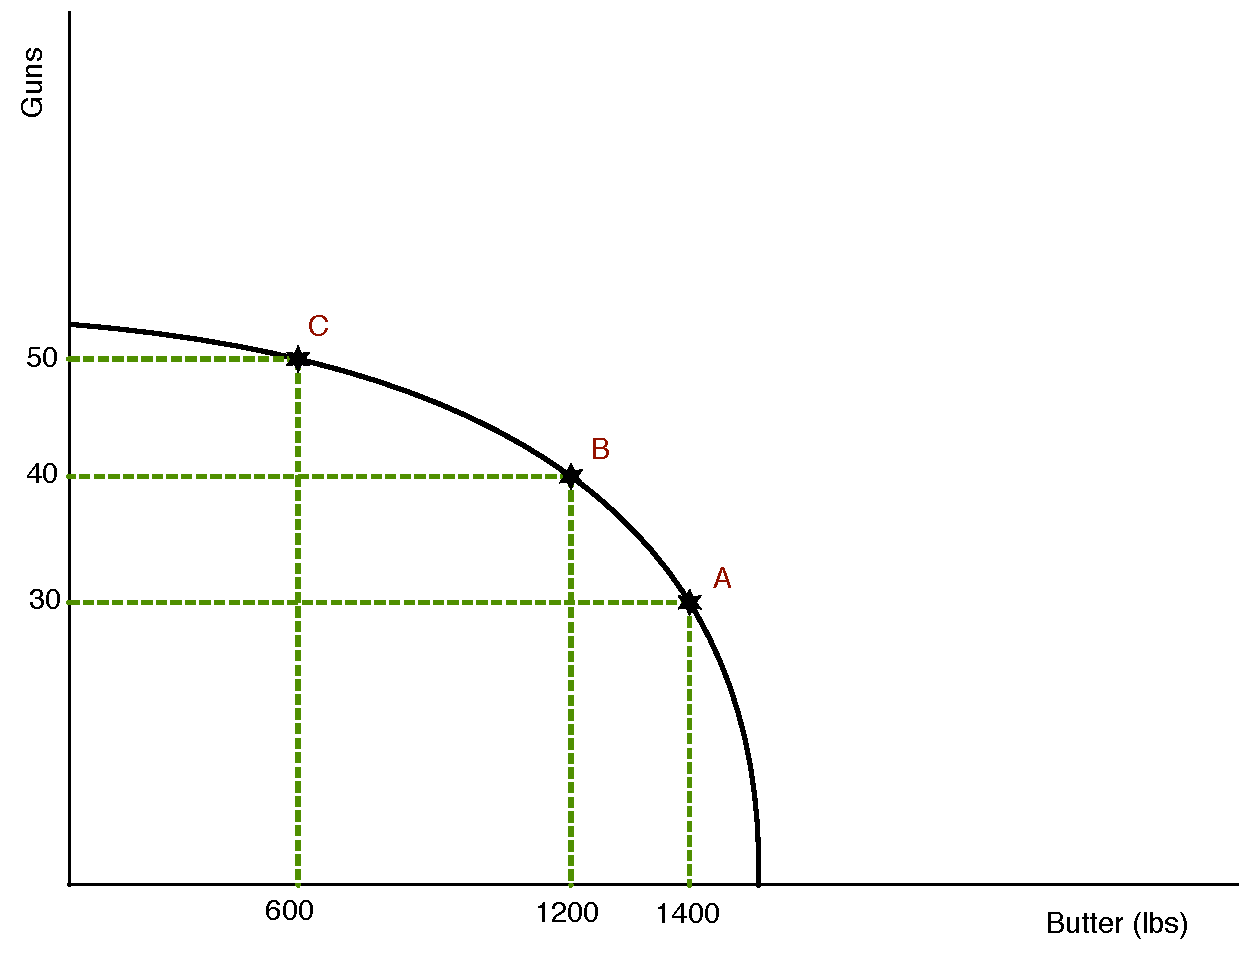
\includegraphics[scale=.25]{Exam_Review2.pdf}
\end{figure}

\pause
\begin{flushright}
	\color{red} 200 lbs of butter; 600 lbs of butter
\end{flushright}

\end{frame}

\begin{frame}{Trade}
	
The table below shows the output per person per day in the US and Japan, who make either drugs or TVs. Assume worker skills are not specialized. 

\begin{table}
	\begin{tabular}{c| c |c }
		 & Drugs & TVs  \\
		\hline 
		US & 2 & 10 \\ 
		Japan & 1 & 3 \\
	\end{tabular}
\end{table}

What is the opportunity cost of producing one TV in each country?

\pause
\begin{flushright}
	\color{red} US. 1 TV: 1/5 drugs; Japan. 1 TV: 1/3 drugs
\end{flushright}

\pause 
What is the expected trade pattern? 
\pause
\begin{flushright}
	\color{red} The US will export TVs to Japan and import drugs.
\end{flushright}

\end{frame}

\begin{frame}
	
How many of the following terms of trade would be acceptable to the US, but not Japan? Which would be acceptable to both?

\begin{enumerate}[(i)]
	\item 10 TVs : 20 drugs
	\item 45 TVs: 180 drugs
	\item 50 TVs: 300 drugs
	\item 60 TVs : 10 drugs 
\end{enumerate}
\vspace{1.5cm}

\pause
\begin{flushright}
	\color{red} 3; None
\end{flushright}

\end{frame}

\begin{frame}{Supply and Demand}
	
\begin{itemize}
	\item Suppose ramen noodles are an inferior good. If incomes increase, then the equilibrium price of ramen noodles will \underline{\hspace{2cm}} and the equilibrium quantity will \underline{\hspace{2cm}}.
	\pause
	\begin{flushright}
		
		\item 	\color{red} decrease; decrease
		
	\end{flushright}
	\pause
	\item Hot dog buns and hot dogs are complements. If the price of hot dogs decreases, then demand for hot dog buns will \underline{\hspace{2cm}} causing a(n) \underline{\hspace{2cm}} in the equilibrium price and a(n) \underline{\hspace{2cm}} in the equilibrium quantity of hot dog buns.
	
	\pause
	\begin{flushright}
		
		\item 	\color{red} increase; increase; increase
		
	\end{flushright}
	
\end{itemize}

\end{frame}

\begin{frame}{Supply and Demand}
	
	\begin{itemize}
		\item Consider the market for orange juice. A drought hits Florida, causing the price of oranges to increase. As a result, there will be a decrease in the \underline{\hspace{2cm}} of orange juice. Before prices are able to adjust, there will be a \underline{\hspace{2cm}} of orange juice at the original market price. Thus, there will be \underline{\hspace{2cm}} pressure on prices.
		\pause
		\begin{flushright}
			
			\item 	\color{red} supply; shortage; upward
			
		\end{flushright}
		\pause
		\item Is the following statement true or false?\\
		``Increased demand for cookies has resulted in higher prices. Due to higher prices, the supply of cookies increases.''
		
		\pause
		\begin{flushright}
			
			\item 	\color{red} False
		\end{flushright}
		
	\end{itemize}
	
\end{frame}

\begin{frame}{Welfare}
	
What is the consumer surplus realized in the market below? The producer surplus?
\\
If a shift in demand caused the price to increase to \$25, what is the change in PS?

\begin{figure}[H]
	\centering
	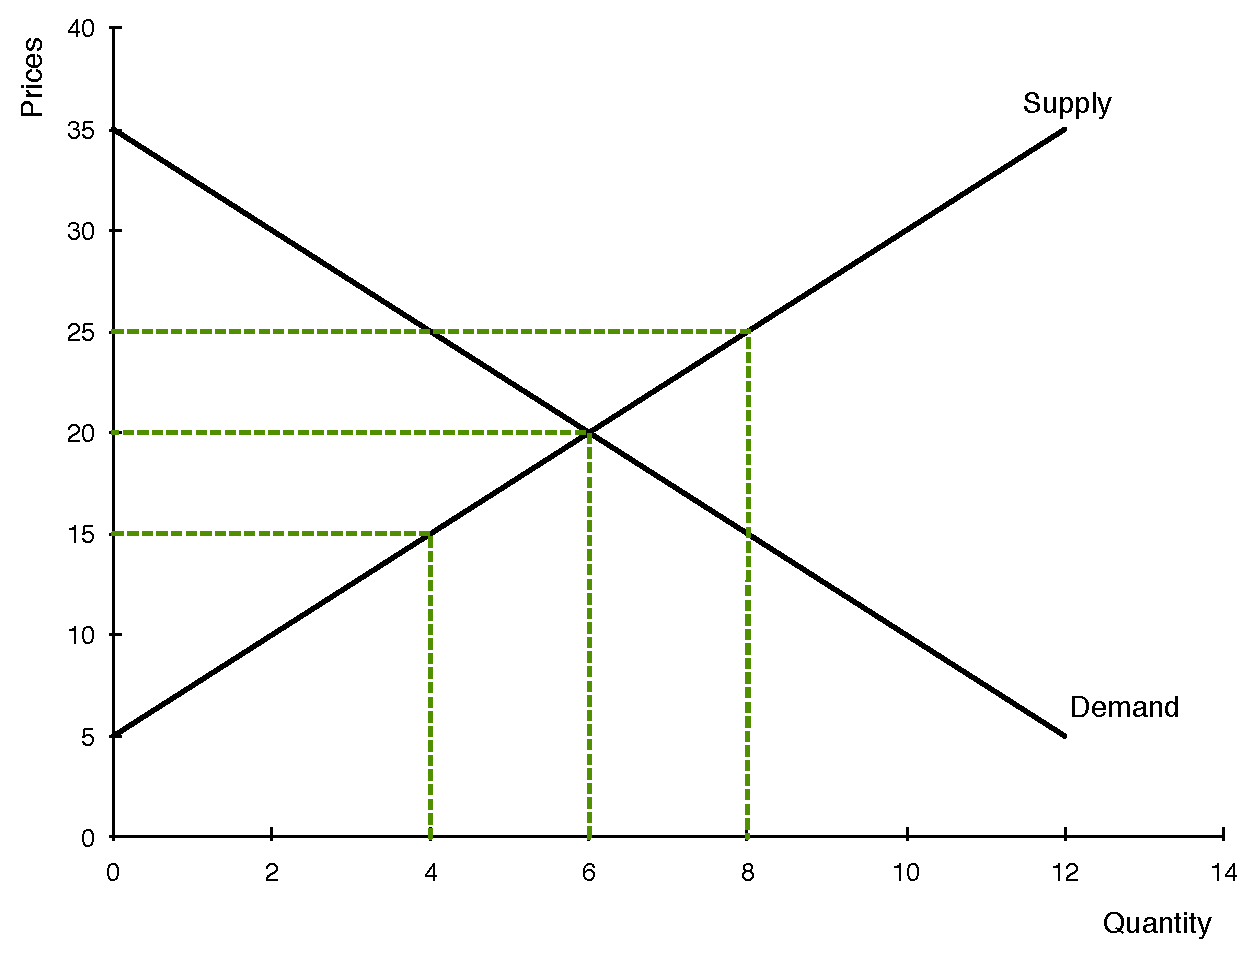
\includegraphics[scale=.25]{Exam_Review3.pdf}
\end{figure}

\pause
\begin{flushright}
	
	\color{red} CS = \$45; PS = \$45
	\\
	PS increases by \$35.
\end{flushright}
	
\end{frame}

\begin{frame}{Elasticity}
	
The supply of beachfront properties is inelastic and the supply of new cars is elastic. Suppose population growth causes demand for both goods to double.

\begin{enumerate}
	\item For which good will price change the most?
	
	\pause
	\begin{flushright}
		
		\color{red} Beachfront property
	\end{flushright}
	
	\pause 
	\item For which good will quantity change the most?
	
	\pause
	\begin{flushright}
		
		\color{red} New cars
	\end{flushright}
	
\end{enumerate}
	
\end{frame}

\begin{frame}{Elasticity}
	
	\begin{enumerate}
		\item 	Cab rides have an income elasticity of demand of $-1.25$. Additionally, the cross-price elasticity of demand between cab rides and the subway is 2. Would an increase in income and a decrease in the price of subway tickets unambiguously decrease the demand for cab rides? 
		
		\pause
		\begin{flushright}
			
			\color{red} Yes
		\end{flushright}
		
		\pause 
		
		\item The price of good $X$ decreases by 6\%. Due to this, the quantity supplied of this good decreases from 10 to 5. What is the price elasticity of supply? 
		
		\pause
		\begin{flushright}
			
			\color{red} 11.11
		\end{flushright}
		
	\end{enumerate}
	
\end{frame}

\begin{frame}{Government Policy}
	
There are 11 buyers and 11 sellers in a used textbook market. Each seller has one book to sell and each buyer wants to buy a book. 

\begin{table}[ht]
	\centering
	\begin{tabular}{ c | c }        
		
		Buyer values   & Seller costs \\
		\hline
		\$51 & \$32 \\
		\$48 & \$17 \\
		\$53 & \$43 \\
		\$40 & \$10 \\
		\$58& \$21 \\
		\$35 & \$45 \\
		\$43 & \$36 \\
		\$55 & \$13 \\
		\$60 & \$28 \\
		\$38 & \$40 \\
		\$45 & \$25 
	\end{tabular}
\end{table}

\end{frame}

\begin{frame}

\begin{enumerate}

\item What is the equilibrium price and quantity in the market?

	\pause
	\begin{flushright}
		
		\color{red} \$40; 9
	\end{flushright}
	
\pause

\item Suppose the government imposes a price ceiling of \$28 on used textbooks. What is the equilibrium quantity and the size of the deadweight loss?

	\pause
	\begin{flushright}
		
		\color{red} $P_C = \$28$; $Q_c= 6$; DWL = \$20 (lost gains from trade).
	\end{flushright}

\end{enumerate}

\end{frame}

\begin{frame}
	
	\begin{figure}[H]
		\centering
		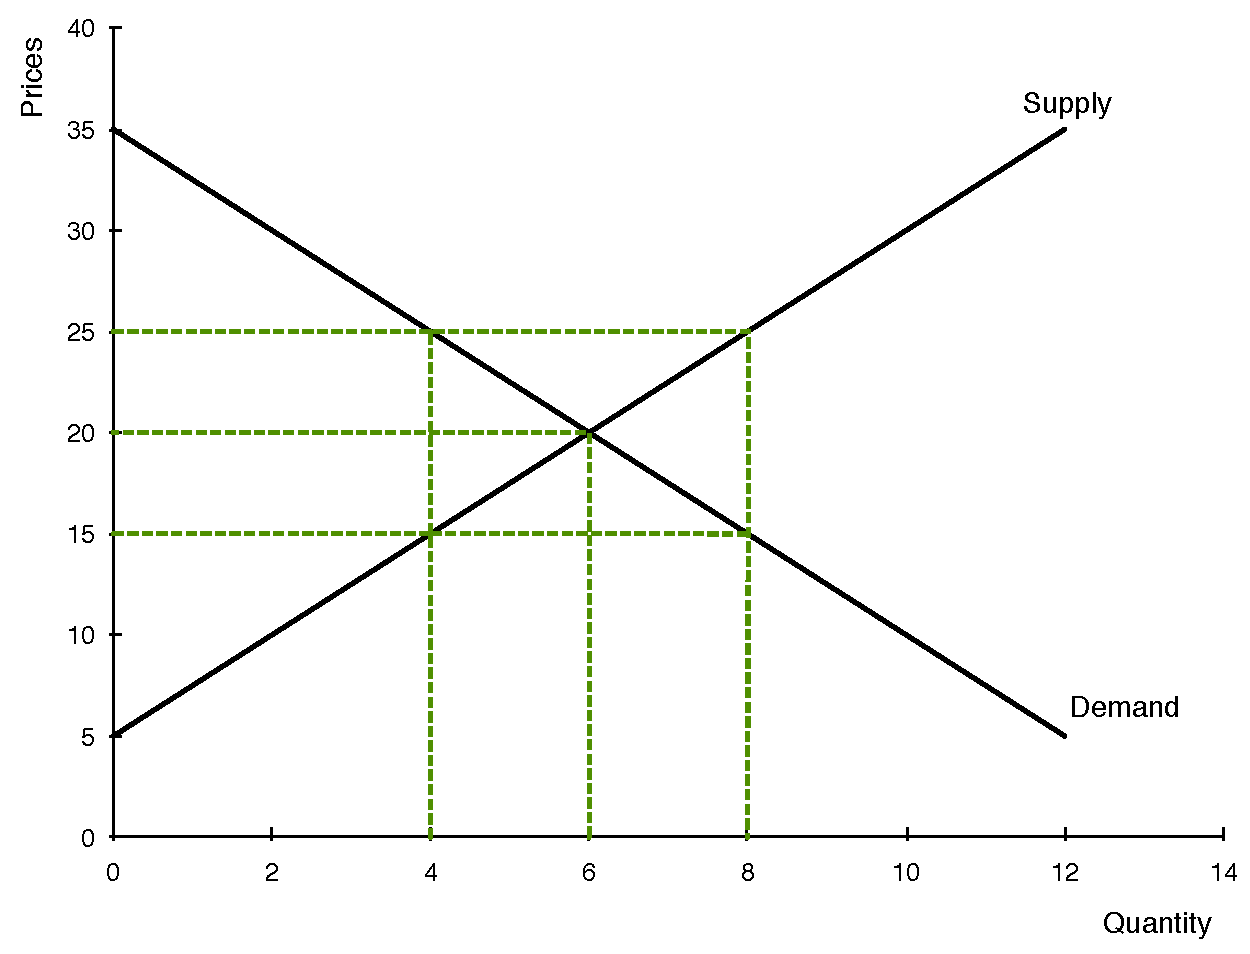
\includegraphics[scale=.20]{Exam_Review4.pdf}
	\end{figure}

	
	If a price ceiling of \$25 is imposed, the DWL in this market would be \underline{\hspace{2cm}}.
	
	\pause
		\begin{flushright}
			
			\color{red} \$0
			
		\end{flushright}
		
	\pause
	If a price ceiling of \$15 is imposed, the DWL in this market would be \underline{\hspace{2cm}}.
	
		\pause
		\begin{flushright}
			
			\color{red} \$10
			
		\end{flushright}
	
\end{frame}

\begin{frame}{Externalities}
	
	Consider the figure below.
	
		\begin{figure}[H]
			\centering
			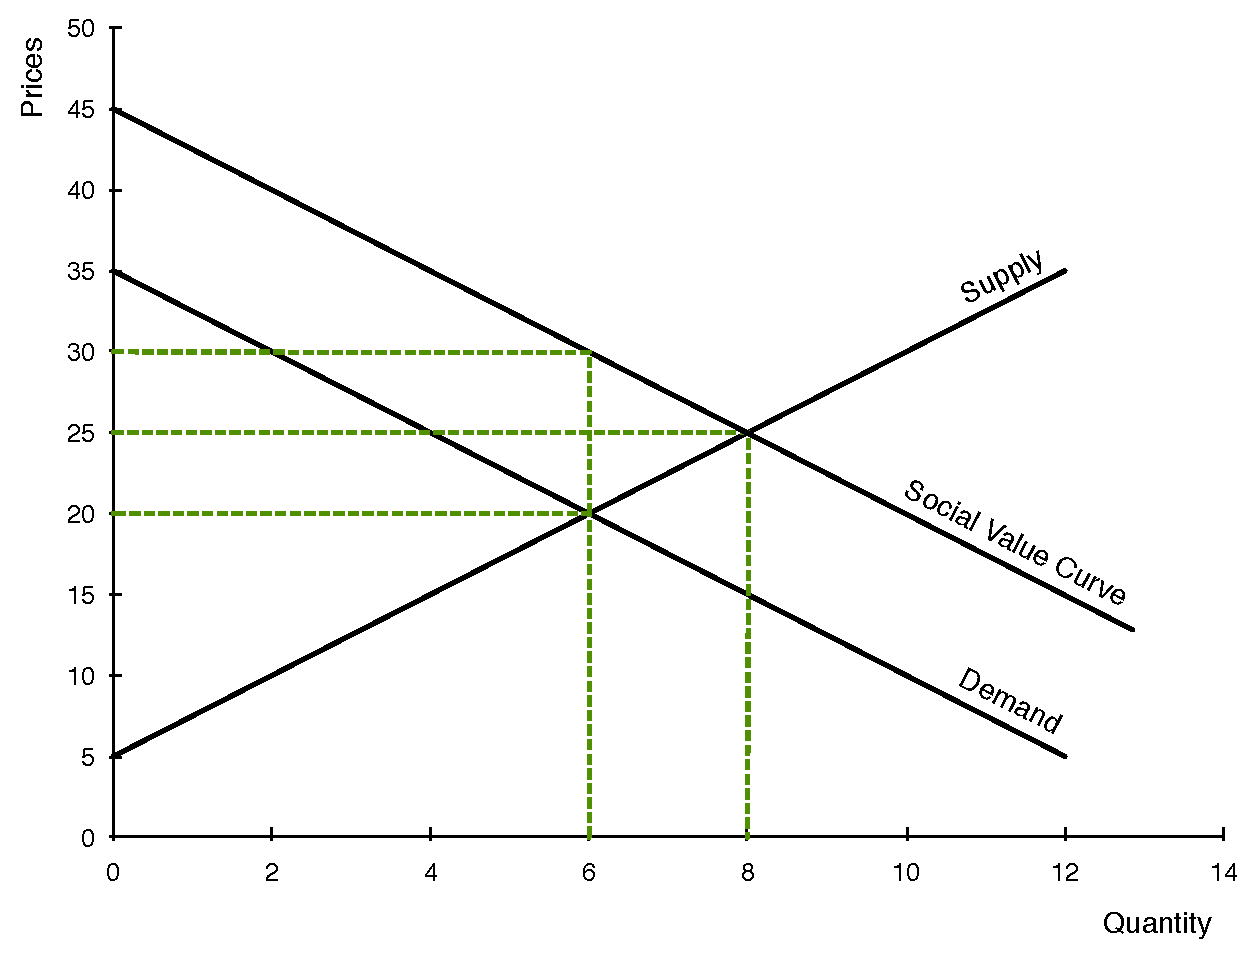
\includegraphics[scale=.20]{Exam_Review5.pdf}
		\end{figure}
		
	What is the external benefit per transaction in this market?
	
	\pause
	\begin{flushright}
		
		\color{red} \$10
		
	\end{flushright}
	
	\pause
	The total external benefit realized at the market equilibrium is \underline{\hspace{2cm}}.
	
	\pause
	\begin{flushright}
		
		\color{red} \$60
		
	\end{flushright}
	

\end{frame}

\begin{frame}
	
	\begin{figure}[H]
		\centering
		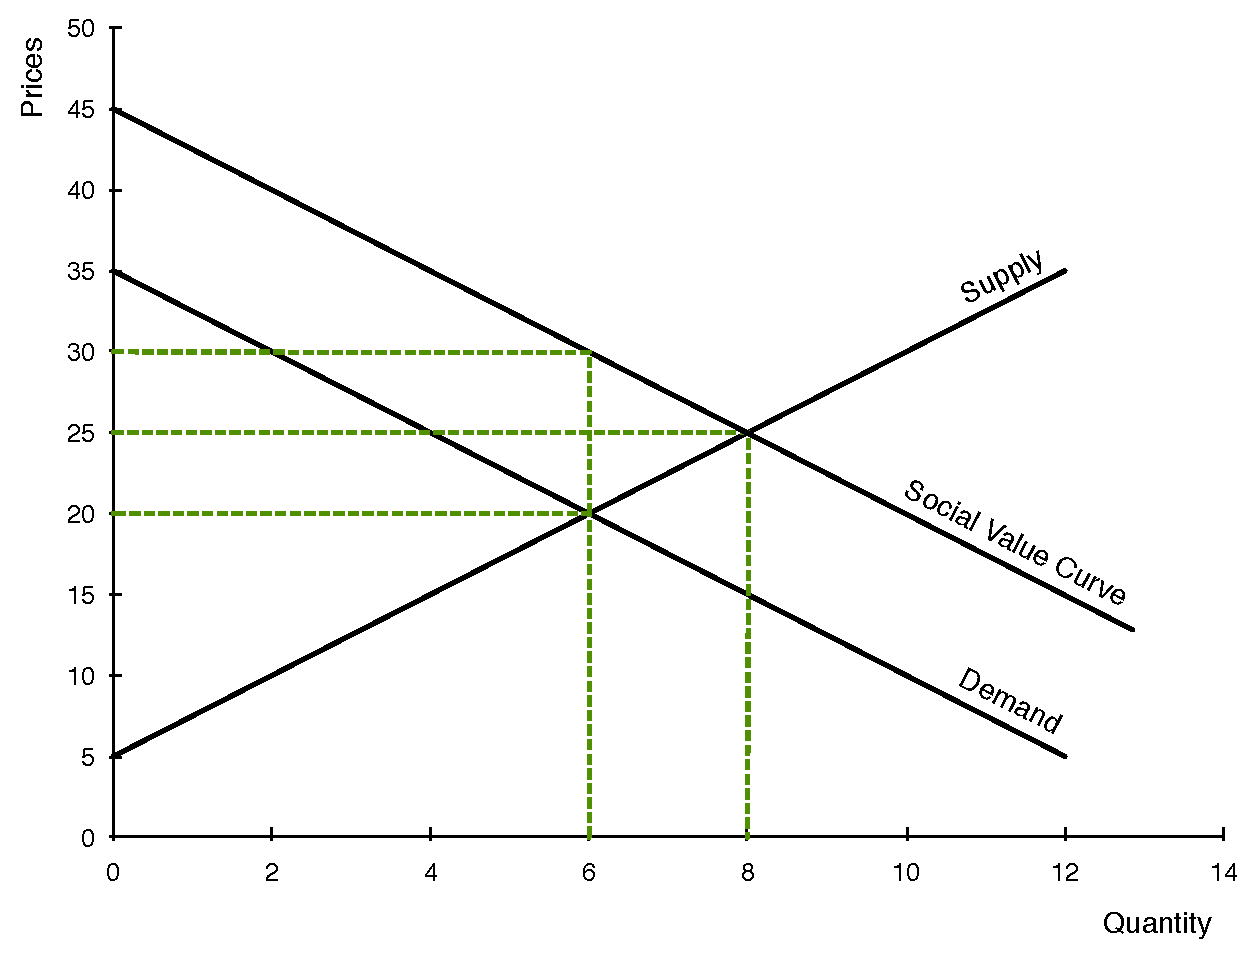
\includegraphics[scale=.25]{Exam_Review5.pdf}
	\end{figure}
	
	What is the deadweight loss in this market?
	
	\pause
	\begin{flushright}
		
		\color{red} \$10
		
	\end{flushright}
	
	\pause
	The socially efficient quantity to produce is \underline{\hspace{2cm}}.
	
	\pause
	\begin{flushright}
		
		\color{red} 8
		
	\end{flushright}
	
\end{frame}


\begin{frame}{Perfect Competition}
	
The table below shows the cost structure of a firm in a perfectly competitive market. 

\begin{table}[ht]
	\centering
	\begin{tabular}{ c | c }        
		
		Quantity of Output & Total Costs \\
		\hline
		0 & \$30\\
		1 & 33 \\
		2 & 38 \\
		3 & 45 \\
		4 & 54 \\
		5 & 65 \\
		6 & 79  \\
		7 & 93 \\
		
		
	\end{tabular}
\end{table}

If the current market price is \$6, how many units of output will the firm produce? 

\pause
\begin{flushright}
	
	\color{red} 2
	
\end{flushright}
	
\end{frame}

\begin{frame}
	
What will be the firm's profits?

\pause
\begin{flushright}
	
	\color{red} $-\$26$
	
\end{flushright}

\pause

What will the firm do in the long run?
	
\pause
\begin{flushright}
	
	\color{red} Exit the market
	
\end{flushright}	

\pause

What will be the long run market price?

\pause
\begin{flushright}
	
	\color{red} \$13
	
\end{flushright}	

	
\end{frame}

\begin{frame}
	\begin{center}
	
	And remember gang, if you think this stuff is hard...
	
	\pause
	
		\begin{figure}[H]
			\centering
			
\includegraphics[scale=.15]{YIKYAK1.png}
		\end{figure}

	
	
		you are not alone.
	\end{center}
	
\end{frame}


\end{document}